\documentclass[aspectratio=169,11pt]{beamer}
\usetheme{Madrid}

\usepackage[utf8]{inputenc}
\usepackage[T1]{fontenc}
\usepackage{lmodern}
\usepackage[spanish]{babel}
\usepackage{amsmath,amssymb}
\usepackage{booktabs}
\usepackage{tikz}
\usepackage{pgfplots}
\usepackage[ruled,vlined]{algorithm2e}
\usetikzlibrary{arrows.meta,positioning}
\pgfplotsset{compat=1.18}

\ifdefined\withnotes
  \setbeameroption{show notes}
\fi

\title[SuperMinHash]{SuperMinHash}
\subtitle{A New Minwise Hashing Algorithm for Jaccard Similarity Estimation}
\author[V.~Hern\'andez \and V.~Wiederhold]{Vicente Hern\'andez \and Vicente Wiederhold}
\institute{An\'alisis de Grandes Vol\'umenes de Datos}
\date{\today}

\setbeamertemplate{navigation symbols}{}
\setbeamertemplate{footline}{%
  \leavevmode%
  \hbox{%
    \begin{beamercolorbox}[wd=.65\paperwidth,ht=2.5ex,dp=1ex,leftskip=1em]{author in head/foot}%
      \usebeamerfont{author in head/foot}SuperMinHash \textperiodcentered{} O.~Ertl (2017)%
    \end{beamercolorbox}%
    \begin{beamercolorbox}[wd=.35\paperwidth,ht=2.5ex,dp=1ex,rightskip=1em,right]{date in head/foot}%
      \usebeamerfont{date in head/foot}\insertshortdate{}\hspace{2em}\insertframenumber/\inserttotalframenumber%
    \end{beamercolorbox}%
  }%
  \vskip0pt%
}

\SetAlgorithmName{Algoritmo}{Algoritmo}{Lista de algoritmos}
\SetKwInput{Entrada}{Entrada}
\SetKwInput{Salida}{Salida}
\SetKw{Ret}{retorna}
\DontPrintSemicolon

\begin{document}

% ---------------------------------------------------------------- 1
\begin{frame}
  \titlepage
  \vspace{0.4em}
  \centering
  {\footnotesize
    \textbf{Autor:} Otmar Ertl \textperiodcentered{} \textbf{Año:} 2017\\
    \textbf{Publicación:} preprint en arXiv (arXiv:1706.05698 [cs.DS]);\\
    no registra publicación en revista o conferencia}
\end{frame}
\note{Presento el trabajo de Otmar Ertl, difundido como preprint en arXiv en 2017.
El objetivo es explicar por que SuperMinHash puede reemplazar a MinHash: mismo
estimador, una sola pasada, menos tiempo para conjuntos grandes y menos varianza
para conjuntos pequenos.}

% ---------------------------------------------------------------- 2
\begin{frame}{Problema y motivación}
  \begin{block}{Problema que aborda el paper}
    Construir firmas compactas de conjuntos que permitan estimar su similitud
    de Jaccard con poco tiempo y memoria, incluso cuando hay muchos conjuntos
    o estos no caben completos en memoria.
  \end{block}
  \begin{itemize}
    \item MinHash estima Jaccard comparando firmas, pero construir una firma
          requiere $O(nm)$ operaciones: $n$ elementos y $m$ posiciones.
    \item Al procesar grandes colecciones, este costo se repite para cada
          conjunto y se vuelve un cuello de botella.
    \item \textbf{Motivación:} reducir el costo y mejorar la precisión,
          manteniendo una sola pasada sobre los datos.
  \end{itemize}
  \vfill
  \centering
  \textbf{Aplicación:} búsqueda de similitud y deduplicación de documentos
  representados como conjuntos de shingles.
\end{frame}
\note{El paper no propone por si solo un sistema completo de deduplicacion.
Aborda una pieza de ese sistema: calcular firmas para estimar Jaccard. Esto es
relevante porque, cuando hay muchos conjuntos o muchos elementos, construir
firmas MinHash puede ser costoso. Ertl busca bajar ese costo y mejorar la
precision, sin perder la propiedad de una sola pasada.}

% ---------------------------------------------------------------- 3
\begin{frame}{El punto de partida: Jaccard y MinHash}
  \small
  \begin{columns}[T]
    \begin{column}{0.44\textwidth}
      \textbf{Similitud de Jaccard}
      \[
        J(A,B)=\frac{|A\cap B|}{|A\cup B|}
      \]
      \begin{itemize}
        \item $A,B$ son conjuntos de elementos (p.\ ej., shingles);
              $J=0$: disjuntos, $J=1$: id\'enticos.
      \end{itemize}
      \vspace{0.2em}
      \textbf{MinHash}
      \[
        h_j(D)=\min_{d\in D} r_j(d),\quad j=0,\ldots,m-1
      \]
      \begin{itemize}
        \item $r_j$: hashes independientes y uniformes en $[0,1)$;
              $m$: tama\~no de la firma.
      \end{itemize}
    \end{column}
    \begin{column}{0.54\textwidth}
      \begin{block}{Estimador}
        \[
          \widehat J=\frac1m\sum_{j=0}^{m-1}\mathbf 1[h_j(A)=h_j(B)]
        \]
      \end{block}
      \begin{itemize}
        \item Insesgado: $\mathbb E[\widehat J]=J$.
        \item Varianza: $\operatorname{Var}(\widehat J)=\dfrac{J(1-J)}{m}$.
        \item Entradas $h_0,\ldots,h_{m-1}$ independientes.
        \item Costo: $O(nm)$, con $n=|D|$.
      \end{itemize}
    \end{column}
  \end{columns}
\end{frame}
\note{Recuerdo las dos piezas basicas. Jaccard mide similitud de conjuntos.
MinHash toma el minimo de m hashes independientes; dos conjuntos coinciden en
una coordenada con probabilidad J, de ahi el estimador. Su varianza baja como
1/m y su costo es O(nm), que es el cuello de botella cuando m es grande.}

% ---------------------------------------------------------------- 3
\begin{frame}{Por qu\'e buscar una alternativa}
  \begin{itemize}
    \item \textbf{MinHash:} $O(nm)$ por firma. Con $m$ grande, el recorrido
          interno domina el costo.
    \item \textbf{One Permutation Hashing} (Li, Owen y Zhang, 2012):
          $O(n+m)$, pero con $|D|<m$ muchos bins quedan vac\'ios.
          La densificaci\'on recupera el estimador, pero pierde precisi\'on;
          adem\'as, tras densificar no se pueden unir firmas.
    \item \textbf{Fast Similarity Sketching} (Dahlgaard et al., 2017):
          $O(n+m\log m)$ y mejor varianza, pero requiere varias pasadas
          (no es streaming) y cuesta cerca del doble que MinHash en conjuntos
          peque\~nos.
  \end{itemize}
  \vfill
  \begin{block}{La pregunta de Ertl (2017)}
    \centering
    \small
    \begin{tabular}{l}
      \textquestiondown Podemos tener \textbf{una sola pasada}, \\
      \textbf{mejor precisi\'on en conjuntos peque\~nos} y \\
      \textbf{menos tiempo} que MinHash para conjuntos grandes?
    \end{tabular}
  \end{block}
\end{frame}
\note{Las alternativas existentes mejoran una parte pero sacrifican otra.
One Permutation Hashing es rapido pero sufre con conjuntos pequenos.
Fast Similarity Sketching tiene mejor precision, pero necesita varias pasadas
y es caro en conjuntos pequenos. La pregunta que motiva el paper es si se
pueden conseguir las tres cosas a la vez.}

% ---------------------------------------------------------------- 4
\begin{frame}{La idea central: una permutaci\'on por elemento}
  \small
  \begin{columns}[T]
    \begin{column}{0.55\textwidth}
      \[
        h_j(D)=\min_{d\in D}\bigl(r_j(d)+\pi_j(d)\bigr)
      \]
      \begin{itemize}
        \item $r_j(d)\sim U[0,1)$.
        \item $\pi_j(d)$ es una permutaci\'on aleatoria de
              $\{0,\ldots,m-1\}$, generada por elemento con
              Fisher--Yates; $h_j(D)\in[0,m)$.
        \item Los valores $r_j(d)+\pi_j(d)$ siguen siendo uniformes e
              independientes entre elementos.
      \end{itemize}
      \vspace{0.3em}
      \begin{block}{Consecuencia}
        \small
        $P(h_j(A)=h_j(B))=J$: el estimador sigue siendo insesgado, pero las
        entradas ya \textbf{no} son independientes.
      \end{block}
    \end{column}
    \begin{column}{0.43\textwidth}
      \centering
      \small
      \textbf{Ejemplo con $m=3$}\\[0.6em]
      \begin{tabular}{c|ccc}
        \toprule
         & $j=0$ & $j=1$ & $j=2$\\
        \midrule
        $d_1$ & $2{,}2$ & $0{,}2$ & $1{,}2$\\
        $d_2$ & $1{,}5$ & $2{,}5$ & $0{,}5$\\
        $d_3$ & $0{,}7$ & $1{,}7$ & $2{,}7$\\
        \midrule
        $h(D)$ & $\mathbf{0{,}7}$ & $\mathbf{0{,}2}$ & $\mathbf{0{,}5}$\\
        \bottomrule
      \end{tabular}
      \vspace{0.5em}

      \footnotesize
      Cada fila es $r_j(d)+\pi_j(d)$ para un elemento;
      la firma es el m\'inimo por columna.
    \end{column}
  \end{columns}
\end{frame}
\note{Aqui esta el cambio conceptual. En vez de m hashes independientes por
elemento, se genera una permutacion aleatoria por elemento y se le suma un
valor uniforme. El minimo por coordenada sigue dando un estimador insesgado
de Jaccard. El ejemplo muestra tres elementos y como se toma el minimo de cada
columna. La diferencia crucial es que las coordenadas de la firma quedan
correlacionadas; eso es lo que despues reduce la varianza.}

% ---------------------------------------------------------------- 5
\begin{frame}{De la definici\'on al algoritmo eficiente}
  \begin{enumerate}
    \item \textbf{Algoritmo directo:} para cada elemento, generar la
          permutaci\'on completa y actualizar las $m$ posiciones.
          Sigue siendo $O(nm)$.
          \medskip
    \item \textbf{Fusionar los bucles y evitar reinicializar:} mantener
          $p$ (la permutaci\'on actual) y $q$ (una marca del elemento que
          inicializ\'o cada posici\'on). As\'i no se reconstruye
          $p$ desde cero en cada iteraci\'on.
          \medskip
    \item \textbf{Usar la permutaci\'on inversa:} actualizar
          $h_{p_j}$ en lugar de $h_j$. Como $r+j$ es estrictamente creciente
          en $j$, los candidatos a mejora aparecen en orden.
          \medskip
    \item \textbf{Salida temprana:} mantener un histograma $b$ de las partes
          enteras de las $h_j$ y el mayor \'indice no vac\'io $a$.
          Si $j>a$, ninguna $h_j$ puede mejorar: se abandona el bucle interno.
  \end{enumerate}
  \vfill
  \begin{block}{Resultado}
    \centering
    \small
    El \textbf{Algoritmo 4} del paper. Para $n\gg m$, el n\'umero esperado de
    iteraciones internas por elemento tiende a \textbf{1}.
  \end{block}
\end{frame}
\note{El algoritmo no sale de la nada: es una cadena de optimizaciones sobre
la definicion. Primero se evita regenerar la permutacion completa. Luego se
trabaja con la permutacion inversa y se explota que r+j crece con j. Finalmente
se usa un histograma de las partes enteras para saber hasta donde puede haber
mejoras. Cuando j supera el maximo indice no vacio a, se corta el bucle.}

% ---------------------------------------------------------------- 6
\begin{frame}[fragile]{Algoritmo 4: el n\'ucleo del m\'etodo}
  \footnotesize
  \textbf{Entrada:} $d_0,\ldots,d_{n-1}$; tama\~no de firma $m$
  \textperiodcentered{}
  \textbf{Salida:} $(h_0,\ldots,h_{m-1})\in[0,m)^m$
  \vspace{-0.3em}
  \begin{algorithm}[H]
    \scriptsize\linespread{0.88}\selectfont
    $(h_0,\ldots)\gets(\infty,\ldots)$;\quad
    $(p_0,\ldots)\gets(0,\ldots,m-1)$;\quad
    $(q_0,\ldots)\gets(-1,\ldots)$\;
    $(b_0,\ldots,b_{m-1})\gets(0,\ldots,0,m)$;\quad $a\gets m-1$\;
    \For{$i\gets0$ \KwTo $n-1$}{
      sembrar el PRNG con $d_i$;\quad $j\gets0$\;
      \While{$j\le a$}{
        $r\sim U[0,1)$;\quad $k\sim U\{j,\ldots,m-1\}$\;
        \lIf{$q_j\ne i$}{$q_j\gets i$;\; $p_j\gets j$}
        \lIf{$q_k\ne i$}{$q_k\gets i$;\; $p_k\gets k$}
        intercambiar $p_j$ y $p_k$\;
        \If{$r+j<h_{p_j}$}{
          $j'\gets\min(\lfloor h_{p_j}\rfloor,m-1)$;\quad
          $h_{p_j}\gets r+j$\;
          \If{$j<j'$}{
            $b_{j'}\gets b_{j'}-1$;\quad $b_j\gets b_j+1$\;
            \While{$b_a=0$}{$a\gets a-1$}
          }
        }
        $j\gets j+1$\;
      }
    }
    \Ret{$(h_0,\ldots,h_{m-1})$}
  \end{algorithm}
\end{frame}
\note{No hay que memorizar el pseudocodigo. Lo importante es reconocer las
tres estructuras auxiliares: p mantiene la permutacion, q evita reinicializar
posiciones que ya se tocaron para el elemento actual, y b con a permite cortar
el while. La condicion del while es j menor o igual a a. Si j supera a a, ya no
puede aparecer una actualizacion que mejore la firma.}

% ---------------------------------------------------------------- 7
\begin{frame}{Ejemplo: mínimos y corte temprano}
  \footnotesize
  \textbf{Firma de tamaño $m=3$:} $h=[h_0,h_1,h_2]$. En cada iteración se
  prueba $r+j$ en la posición elegida por la permutación; se conserva el mínimo.
  Los valores son una ejecución ilustrativa.

  \begin{columns}[T]
    \begin{column}{0.49\textwidth}
      \textbf{Primer elemento:} inicio $h=[\infty,\infty,\infty]$.
      \vspace{0.3em}

      \begin{tabular}{cccc}
        \toprule
        $j$ & $r+j$ & Posición & Resultado \\
        \midrule
        0 & 0,4 & $h_2$ & $h_2\gets0,4$ \\
        1 & 1,2 & $h_0$ & $h_0\gets1,2$ \\
        2 & 2,7 & $h_1$ & $h_1\gets2,7$ \\
        \bottomrule
      \end{tabular}

      \vspace{0.3em}
      Firma: $[1,2;\,2,7;\,0,4]$; partes enteras $[1,2,0]$,
      por tanto $a=2$.
    \end{column}
    \begin{column}{0.49\textwidth}
      \textbf{Siguiente elemento:}
      \begin{itemize}
        \item $j=0$: candidato 0,1 actualiza $h_1$;
              firma $[1,2;\,0,1;\,0,4]$, así que $a=1$.
        \item $j=1$: candidato 1,6 no mejora $h_2=0,4$.
        \item $j=2>a$: para y omite las iteraciones restantes.
      \end{itemize}
      \vspace{0.2em}
      \textbf{Tercer elemento:} $j=0$ actualiza $h_0$ a 0,2; ahora $a=0$,
      por lo que se omiten $j=1,2$.
    \end{column}
  \end{columns}
  \vfill
  \begin{block}{Ahorro en esta ejecución}
    \centering
    3 elementos $\times$ 3 iteraciones posibles = 9;
    SuperMinHash realiza 3+2+1 = \textbf{6 iteraciones}.
  \end{block}
  \scriptsize El histograma mantiene $a$ sin volver a recorrer todas las posiciones.
  Este ejemplo ilustra el mecanismo; no garantiza ese ahorro en cada conjunto.
\end{frame}
\note{Los valores son inventados para mostrar el mecanismo. Tras el primer
elemento, las partes enteras de la firma son 1, 2 y 0, así que a vale 2. El
segundo elemento baja h1 de 2,7 a 0,1; desaparece el rango 2 y a baja a 1. En
j=1 no hay mejora. Al llegar a j=2, los candidatos son al menos 2 y todas las
posiciones ya son menores que 2, así que el resto se omite. El tercer elemento
baja h0 y hace que a llegue a 0, permitiendo cortar después de j=0. En esta
ejecución se hacen seis iteraciones en lugar de nueve; es solo una ilustración,
no una garantía universal.}

% ---------------------------------------------------------------- 8
\begin{frame}{Precisi\'on: menos varianza para conjuntos peque\~nos}
  \footnotesize
  \[
    \widehat J=\frac1m\sum_{j=0}^{m-1}\mathbf 1[h_j(A)=h_j(B)],
    \qquad
    \operatorname{Var}(\widehat J)=\frac{J(1-J)}{m}\,\alpha(m,u)
  \]
  \[
    \alpha(m,u)=1-
    \frac{\displaystyle\sum_{l=1}^{m-1} l^{u}\bigl((l+1)^{u}+(l-1)^{u}-2l^{u}\bigr)}
         {\displaystyle (m-1)^{u-1}\,m^{u}\,(u-1)},
    \qquad u=|A\cup B|
  \]
  \begin{columns}[T]
    \begin{column}{0.52\textwidth}
      \begin{itemize}
        \item $\alpha(m,u)\in[0,1)$: factor de reducci\'on frente a MinHash.
        \item S\'olo depende de $m$ y de $u=|A\cup B|$; \textbf{no} de $J$.
        \item Si $u<m$, la varianza es aproximadamente la mitad.
        \item Si $u\gg m$, $\alpha\to1$: la ventaja desaparece.
        \item La mejora viene de la dependencia entre entradas, no de m\'as
              hashes.
      \end{itemize}
    \end{column}
    \begin{column}{0.46\textwidth}
      \centering
      \begin{tikzpicture}
        \begin{axis}[
            width=6.3cm, height=4.4cm,
            xmode=log, log basis x=2,
            xmin=2, xmax=4096, ymin=0.3, ymax=1.02,
            xlabel={$u=|A\cup B|$}, ylabel={$\alpha(m,u)$},
            xtick={2,8,32,128,512,2048},
            xticklabels={2,8,32,128,512,2048},
            ytick={0.4,0.6,0.8,1.0},
            grid=major, grid style={gray!18},
            tick label style={font=\tiny},
            label style={font=\scriptsize},
            legend style={font=\tiny, at={(0.98,0.02)}, anchor=south east,
                          draw=none, fill=none},
          ]
          \addplot[thick, blue] table[x=u,y=m8] {data/alpha.dat};
          \addlegendentry{$m=8$}
          \addplot[thick, teal] table[x=u,y=m16] {data/alpha.dat};
          \addlegendentry{$m=16$}
          \addplot[thick, orange] table[x=u,y=m32] {data/alpha.dat};
          \addlegendentry{$m=32$}
          \addplot[thick, red] table[x=u,y=m64] {data/alpha.dat};
          \addlegendentry{$m=64$}
          \addplot[thick, purple] table[x=u,y=m128] {data/alpha.dat};
          \addlegendentry{$m=128$}
        \end{axis}
      \end{tikzpicture}
    \end{column}
  \end{columns}
\end{frame}
\note{La formula de la varianza es el resultado mas importante. El factor alpha
mide cuanto se reduce la varianza respecto de MinHash. Depende solo del tamano
de firma m y de la cardinalidad de la union u, no de J. Para conjuntos pequenos
en comparacion con m, alpha ronda la mitad; para uniones mucho mas grandes que
m, alpha se acerca a 1 y la ventaja se pierde. La figura reproduce la forma de
la funcion del paper.}

% ---------------------------------------------------------------- 8
\begin{frame}{Runtime y comparaci\'on con el estado del arte}
  \centering
  \footnotesize
  \begin{tabular}{lcccc}
    \toprule
    \textbf{Algoritmo} & \textbf{Tiempo} & \textbf{Pasadas} &
    \textbf{Conjuntos peque\~nos} & \textbf{Streaming}\\
    \midrule
    MinHash & $O(nm)$ & 1 & referencia & s\'i\\
    One Permutation Hashing & $O(n+m)$ & 1 & menor precisi\'on & s\'i\\
    Fast Similarity Sketching & $O(n+m\log m)$ & varias & mejor & no\\
    \textbf{SuperMinHash} & $O(n+m\log^2 m)$ & \textbf{1} &
    $\alpha(m,u)<1$ & \textbf{s\'i}\\
    \bottomrule
  \end{tabular}
  \vspace{0.8em}

  \begin{columns}[T]
    \begin{column}{0.54\textwidth}
      \begin{itemize}
        \item $T(n,m)=n+\sum_{s=1}^{m-1}\min(t_s,n)$: $t_s$ es el tiempo de
              coupon collector con grupos de tama\~no $s$.
        \item Cota: $O(n+m\log^2m)$. Amortizado: $\to1$ iteraci\'on por
              elemento cuando $n\to\infty$.
        \item Caso peor: $nm$; los duplicados ordenados pueden activarlo.
      \end{itemize}
    \end{column}
    \begin{column}{0.44\textwidth}
      \begin{block}{En una frase}
        \small
        Nunca usa m\'as iteraciones internas que MinHash; para $n$ grande,
        usa muchas menos. El costo por iteraci\'on es mayor, pero la ventaja
        asint\'otica domina.
      \end{block}
    \end{column}
  \end{columns}
\end{frame}
\note{La tabla resume el posicionamiento. SuperMinHash mantiene una sola
pasada, mejora la precision en conjuntos pequenos y tiene costo
$O(n+m\log^2 m)$. La formula de T suma el costo de insertar n elementos mas el costo de que a
baje desde m-1 hasta 1; eso se modela como coupon collector con grupos. En el
peor caso sigue siendo n*m, y los duplicados ordenados son el caso adversarial.
El paper enfatiza que nunca necesita mas iteraciones internas que MinHash.}

% ---------------------------------------------------------------- 9
\begin{frame}{La evidencia experimental del paper}
  \begin{columns}[T]
    \begin{column}{0.49\textwidth}
      \begin{block}{Precisi\'on (Fig.~1)}
        \footnotesize
        \begin{itemize}
          \item $100\,000$ simulaciones por caso.
          \item Casos con $u=3\cdot2^k$ y $u=4\cdot2^k$, $k=0,\ldots,11$.
          \item Se estima la varianza y se divide por la de MinHash para
                obtener $\alpha$ experimental.
          \item Las cruces coinciden con la f\'ormula (7).
        \end{itemize}
      \end{block}
    \end{column}
    \begin{column}{0.49\textwidth}
      \begin{block}{Runtime (Fig.~2)}
        \footnotesize
        \begin{itemize}
          \item $1\,000$ conjuntos aleatorios.
          \item $n=2^k$, $k=0,\ldots,20$, y $n=3\cdot2^k$,
                $k=0,\ldots,19$.
          \item Iteraciones internas por elemento: empiezan en $m$ y
                tienden a $1$ cuando $n$ crece.
          \item Para $n$ grande, la mejora puede acercarse a un factor $m$.
        \end{itemize}
      \end{block}
    \end{column}
  \end{columns}
  \vfill
  \begin{block}{Implementaci\'on de los experimentos}
    \centering
    \small
    MurmurHash3 de 128 bits con semilla; secuencia predefinida de semillas
    para generar bits pseudoaleatorios.
  \end{block}
  \vspace{0.3em}
  \footnotesize
  El paper valida la teor\'ia con simulaci\'on; no reporta un benchmark
  end-to-end de un pipeline de deduplicaci\'on.
\end{frame}
\note{El paper no solo propone el algoritmo: valida las dos predicciones
centrales. Para la precision simula muchisimos pares de conjuntos con tamanos
controlados y comprueba que la varianza experimental sigue la formula. Para el
runtime mide cuantas iteraciones internas se necesitan en promedio y muestra que
bajan desde m hasta aproximadamente 1. Es una validacion del algoritmo, no un
benchmark de un sistema completo de deduplicacion.}

% ---------------------------------------------------------------- 10
\begin{frame}{Gr\'aficos de los experimentos}
  \begin{columns}[T]
    \begin{column}{0.49\textwidth}
      \centering
      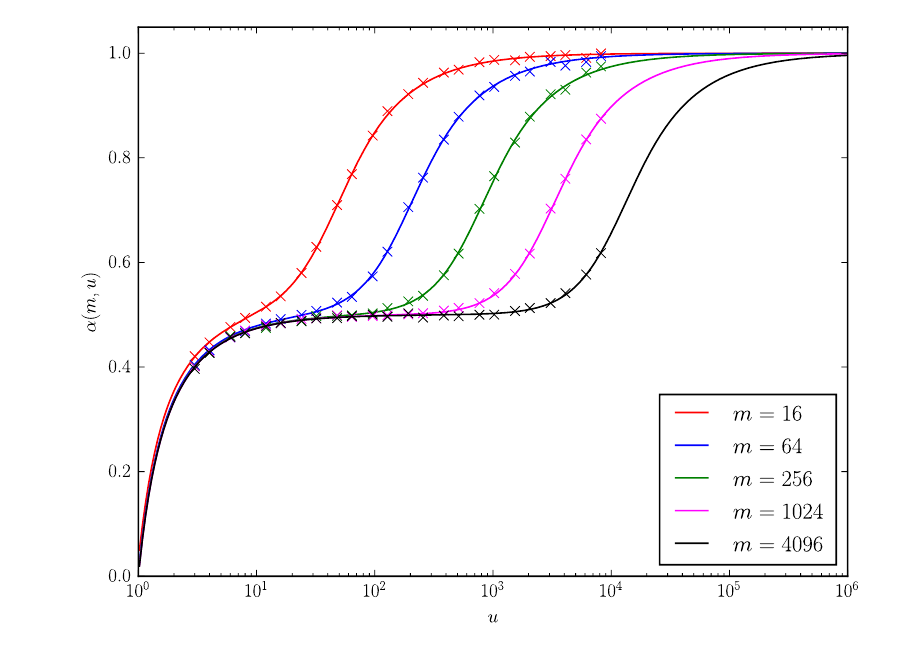
\includegraphics[width=\linewidth,height=0.64\textheight,keepaspectratio]
        {figures/variance-experiment.png}
      \scriptsize
      \textbf{Precisi\'on:} factor $\alpha(m,u)$ de varianza relativa.
      Las cruces son resultados de simulaci\'on; las curvas, la predicci\'on te\'orica.
    \end{column}
    \begin{column}{0.49\textwidth}
      \centering
      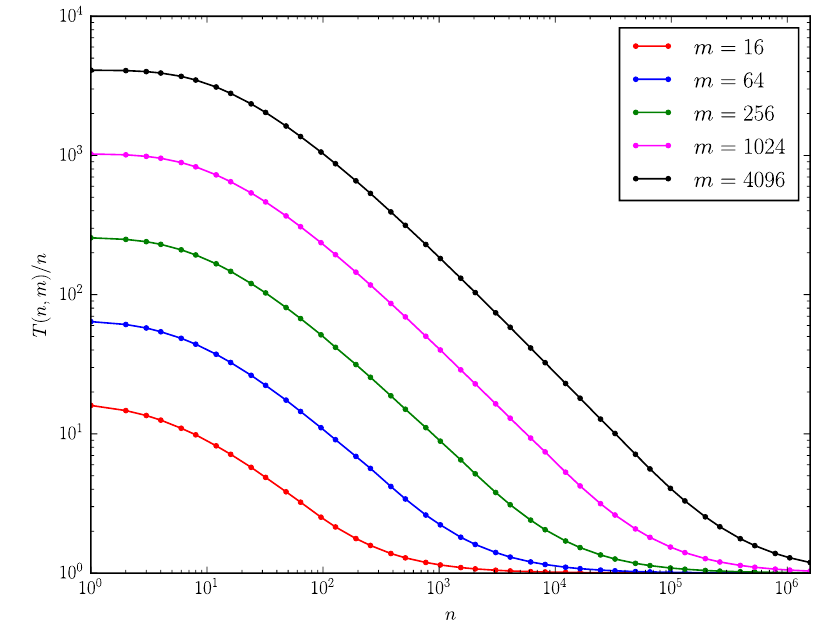
\includegraphics[width=\linewidth,height=0.64\textheight,keepaspectratio]
        {figures/runtime-experiment.png}
      \scriptsize
      \textbf{Runtime:} iteraciones internas promedio por elemento; disminuyen
      hacia 1 a medida que crece el conjunto.
    \end{column}
  \end{columns}
  \vfill
  \centering
  \tiny Figuras 1 y 2 del paper de Ertl (2017).
\end{frame}
\note{Estas son las dos graficas reportadas en el paper. A la izquierda, alpha
es el factor por el que se multiplica la varianza de MinHash: valores menores
significan menor varianza. Las cruces de simulacion concuerdan con las curvas
teoricas. A la derecha, el eje vertical muestra el numero promedio de
iteraciones internas por elemento. Para cada tamano m, el costo empieza cerca
de m cuando hay pocos elementos y se aproxima a una iteracion cuando n crece.
Son resultados del algoritmo de firmas, no de un sistema completo de
deduplicacion.}

% ---------------------------------------------------------------- 11
\begin{frame}{Fortalezas, limitaciones y cr\'itica}
  \begin{itemize}
    \item \textbf{Fortaleza:} reemplazo directo de MinHash: mismo estimador,
          misma interfaz, una sola pasada y mejor precisi\'on en conjuntos
          peque\~nos.
    \item \textbf{La dependencia es arma de doble filo:} mejora la varianza,
          pero el an\'alisis cl\'asico de LSH \emph{banding} supone entradas
          independientes. La curva-S puede desviarse; hay que calibrarla
          emp\'iricamente o generar candidatos con MinHash.
    \item \textbf{Costo oculto:} cada iteraci\'on usa PRNG y enteros aleatorios;
          contar iteraciones no es lo mismo que medir tiempo de pared.
    \item \textbf{Duplicados:} no mejoran el estado; con duplicados ordenados
          el costo puede volver al caso peor $nm$.
    \item \textbf{Tama\~no:} la ganancia de precisi\'on es para $u<m$; si
          $u\gg m$, $\alpha\to1$ y s\'olo queda la mejora de runtime.
  \end{itemize}
  \vfill
  \begin{block}{Para nuestro proyecto}
    \small
    Usarlo como firma principal y comparar contra MinHash; calibrar LSH con
    firmas dependientes y medir tiempo real, no s\'olo iteraciones.
  \end{block}
\end{frame}
\note{Hay que ser criticos. SuperMinHash no es gratis: la dependencia que mejora
la varianza rompe la hipotesis de independencia que se usa normalmente para
analizar LSH. Si se usa banding, hay que medir la curva-S real. Tambien hay un
costo de PRNG que el analisis de iteraciones no captura. Los duplicados son un
caso debil, y la mejora de precision desaparece cuando la union es mucho mas
grande que m. Para el proyecto, la recomendacion es medir ambos esquemas y
calibrar LSH experimentalmente.}

% ---------------------------------------------------------------- 11
\begin{frame}{Conclusiones}
  \begin{enumerate}
    \item \textbf{Mismo estimador, mejor varianza:}
          $\operatorname{Var}(\widehat J)=\frac{J(1-J)}{m}\alpha(m,u)$,
          con $\alpha<1$ y aproximadamente $1/2$ para $u<m$.
    \item \textbf{Mejor runtime:} $O(n+m\log^2m)$ para elementos distintos,
          con costo amortizado cercano a una iteraci\'on interna por elemento.
    \item \textbf{Una sola pasada:} apto para streaming y para datos que no
          caben en memoria.
    \item \textbf{No es magia:} la ganancia depende de la calidad del hash,
          del PRNG, de los duplicados y del r\'egimen de tama\~nos.
  \end{enumerate}
  \vfill
  \begin{block}{Idea para recordar}
    \centering
    \small
    SuperMinHash no calcula m\'as hashes: cambia la forma de construir la
    firma para que las entradas se ayuden entre s\'i y para poder cortar el
    c\'omputo antes.
  \end{block}
\end{frame}
\note{Para cerrar: el paper propone un reemplazo de MinHash que mantiene el
mismo estimador, reduce la varianza en conjuntos pequenos y baja el costo de
calculo para conjuntos grandes, todo en una sola pasada. La clave no es usar
mas hashes, sino construir la firma con permutaciones por elemento y explotar la
estructura para cortar el bucle interno. Las limitaciones practicas son la
dependencia para LSH, el costo del PRNG y los duplicados.}

% ---------------------------------------------------------------- 12
\begin{frame}[allowframebreaks]{Referencias}
  \footnotesize
  \begin{thebibliography}{9}
    \bibitem{ertl} O.~Ertl.
      \emph{SuperMinHash --- A New Minwise Hashing Algorithm for Jaccard
      Similarity Estimation.}
      arXiv:1706.05698 [cs.DS], 2017.

    \bibitem{broder} A.~Z. Broder.
      \emph{On the Resemblance and Containment of Documents.}
      Compression and Complexity of Sequences (SEQUENCES), 1997.

    \bibitem{li} P.~Li, A.~Owen, C.~Zhang.
      \emph{One Permutation Hashing.}
      Advances in Neural Information Processing Systems (NeurIPS), 2012.

    \bibitem{dahlgaard} S.~Dahlgaard, M.~B.~T.~Knudsen, M.~Thorup.
      \emph{Fast Similarity Sketching.}
      arXiv:1704.04370, 2017.

    \bibitem{lumbroso} J.~Lumbroso.
      \emph{Optimal Discrete Uniform Generation from Coin Flips, and
      Applications.}
      arXiv:1304.1916, 2013.
  \end{thebibliography}
\end{frame}
\note{Referencias principales. El paper de Ertl es la fuente de las definiciones,
el algoritmo, la formula de varianza y los experimentos. Broder es el origen de
MinHash; Li et al. y Dahlgaard et al. son las alternativas que el paper compara;
Lumbroso se usa para generar enteros uniformes de forma eficiente.}

% ---------------------------------------------------------------- Backup
\appendix

\begin{frame}{Backup: de la covarianza a $\alpha(m,u)$}
  \small
  Para $j\ne k$, el paper deriva
  \[
    \operatorname{Cov}\bigl(\mathbf 1[h_j(A)=h_j(B)],\,
    \mathbf 1[h_k(A)=h_k(B)]\bigr)
    =J(1-J)\left(-\frac{1-\alpha(m,u)}{m-1}\right).
  \]
  Para $j=k$, la covarianza es $J(1-J)$. Entonces
  \[
    \operatorname{Var}(\widehat J)
    =\frac{1}{m^2}\left[mJ(1-J)-m(m-1)J(1-J)\frac{1-\alpha}{m-1}\right]
    =\frac{J(1-J)}{m}\alpha.
  \]
  La dependencia entre entradas hace que las covarianzas sean negativas y
  reduzcan la suma.
\end{frame}
\note{Esta es la intuicion de la demostracion. Las entradas no son
independientes: los indicadores de coincidencia tienen covarianza negativa para
j distinto de k. Al sumar la varianza, esos terminos negativos reducen el total
y aparece alpha. No hace falta presentar la integral del apendice en la charla;
basta con senalar que la mejora viene de covarianzas negativas.}

\begin{frame}{Backup: detalles de implementaci\'on}
  \begin{itemize}
    \item \textbf{PRNG:} se siembra con cada elemento $d_i$; se consumen bits
          de MurmurHash3 de 128 bits para generar uniformes y permutaciones.
    \item \textbf{Permutaci\'on:} Fisher--Yates; s\'olo se generan las
          posiciones que el corte temprano necesita.
    \item \textbf{Invariantes:} $p$ es la permutaci\'on actual, $q_k=i$
          indica que $p_k$ ya fue inicializado para $d_i$, y $b$ cuenta las
          partes enteras de las $h$.
    \item \textbf{Corte:} $a$ es el mayor \'indice con $b_a>0$; si
          $j>a$, no hay actualizaciones posibles.
    \item \textbf{Duplicados:} si $d_i=d_{i'}$, la segunda inserci\'on no
          cambia el estado; conviene deduplicar antes si el orden es adverso.
  \end{itemize}
\end{frame}
\note{Material de apoyo por si preguntan por la implementacion. Lo importante es
que el algoritmo necesita un generador de enteros uniformes eficiente, porque
genera permutaciones por elemento. Fisher-Yates se puede hacer de forma
perezosa, y el corte temprano evita la mayor parte del trabajo. Los duplicados
no aportan informacion nueva y pueden degradar el runtime.}

\end{document}
